\chapter{Fundamentals of Machine Learning and Neural Networks}
\label{ml-fundamentals}

In modern medicine, 
ever increasing amounts of data 
is continuously being generated and collected.
Ranging from structured administrative data 
used primarily for billing purposes
to advanced imaging and high-througput \enquote{omics} analyses,
the array of available data is as diverse as it is plentiful.
Making sense and making use of such massive amounts of data 
necessitates automated methods for data analysis.

% figure: hierarchy of artificial intelligence {{{
\begin{marginfigure}[3em]
    \centering
	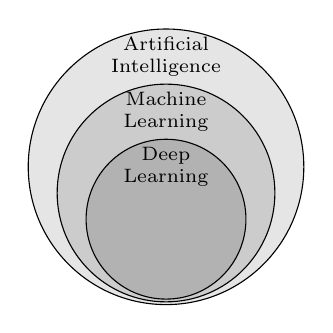
\begin{tikzpicture}[scale=1.75]
        \draw[black, fill=black!10] (0,  0.00) circle (1.00);
        \draw[black, fill=black!20] (0, -0.19) circle (0.79);
        \draw[black, fill=black!30] (0, -0.38) circle (0.58);
        \node[font=\scriptsize, text width=1.8cm, align=center] 
            at (0, 0.8) {Artificial Intelligence};
        \node[font=\scriptsize, text width=1.8cm, align=center] 
            at (0, 0.4) {Machine Learning};
        \node[font=\scriptsize, text width=1.4cm, align=center] 
            at (0, 0.0) {Deep Learning};
	\end{tikzpicture}
    \caption[The hierarchy of artificial intelligence (AI)]{%
        \Ac*{AI} is an umbrella term for computer software 
        that have some sort of \enquote{intelligence} and
        \ac*{ML} is a collection of methods through which 
        that can be achieved. 
        \Ac*{DL}, a specific method in \acs*{ML}, 
        relies on neural networks with many layers
        to analyse complex data.
    }
    \label{fig:artificial-intelligence}
\end{marginfigure}% }}}

\Ac{AI}, and specificically \ac{ML} (\cref{fig:artificial-intelligence}),
seeks to address this need by development of methods and algorithms
that allows computers to \enquote{learn} from data to solve new problems
instead of them being explicitly programmed.
~\autocite{murphyMachine2012}
The field of \ac{ML} have progressed exponentially
over the past couple of decades, 
and with the advent of generative \ac{AI} models like 
GPT-4~\autocite{openaiGPT42023} and
DALL-E~\autocite{rameshZeroShot2021}
there is a growing public interest in the use of \ac{AI} and \ac{ML}.
In the context of precision medicine,
the promise of \ac{AI} lies in the ability 
to integrate large amounts of data from huge data sets
and register and highlight patterns with clinical importance.

The underlying principle of \ac{ML} is to formulate a learning problem with a
well-defined objective and a quantifiable measure of performance.
Subsequently,
a loosely defined computer program is established and fed with data
representing said objective.
Guided by the performance metric, \ac{ML}
algorithms iteratively refine the underlying computer program until the
objective is optimally addressed. 
In his 1997 book \citetitle{mitchellMachine1997},
\citeauthor*{mitchellMachine1997} defines this formally as:
\begin{displayquote}[mitchellMachine1997]
   A computer program is said to learn from experience \(E\)
   with respect to some class of tasks \(T\) and performance measure \(P\),
   if its performance at tasks in \(T\), as measured by \(P\), 
   improves with experience \(E\).
\end{displayquote}
Though this conceptual framework is common to all \ac{ML} models, 
the diversity in \ac{ML} arises from not only the specific \ac{ML} algorithm, 
but also choices regarding objectives, performance metrics, and program attributes. 
These selections introduce the myriad variations and nuances within \ac{ML}, 
which can be broadly categorized into two distinct approaches:
supervised learning
and 
unsupervised learning.

\section{Supervised Learning}

In supervised learning, models are trained on labeled examples---%
a dataset 
\(\mathfrak{D} = \{(\bm{x}_i, \bm{y}_i) \mid i \in \{1, \ldots, N\}\} \) 
of size \(N\) that contains both input data \(\bm{x}\)
and corresponding correct output values \(\bm{y}\). 
Here \( \mathfrak{D} \) is typically refered to as the training set.
~\autocite{murphyMachine2012}
The primary aim in supervised learning 
is to learn a function that correctly 
maps input data to output data, 
i.e. correctly assigns output labels or values
based on the features present in the input data.
When the output is discrete labels or classes, 
the task is called a classification problem.
Conversely, 
if the output is continuous values,
it is called a regression problem.

Illustrating with a supervised learning task in the domain of classification, 
we can consider a database of coronary angiography images that have been 
manually annotated to indicate the presence or absence of critical stenosis 
in any of the coronary arteries. 
In this scenario, 
the output classes are denoted as 
\(\bm{y} \in \{\textsf{stenosis}, \textsf{no stenosis}\}\), 
and the objective is to classify the images 
into either of these categories based on their pixel values.
The labeled data is being used to guide and \enquote{supervise}
the model in order for it accurately accomplish this categorisation.

Two other examples of supervised learning tasks is presented in 
\nameref{chap:paper-2} and 
\nameref{chap:paper-3}
within this thesis.
However, these tasks differ from classical supervised learning
in that they involve time-to-event predictions and censored labels.
This subject matter will be elaborated upon in the next chapter:
\nameref{survival-analysis}.

\section{Unsupervised Learning}

In contrast to supervised learning,
unsupervised learning is concerned with finding 
underlying patterns or structures within unlabeled datasets. 
In this paradigm, the algorithm operates without the aid of 
predetermined labels or categories, instead learning from the data itself. 
The aim is to discover intrinsic structure in the dataset, 
which can then be used for tasks such as 
dimensionality reduction, clustering, or anomaly detection.
~\autocite{murphyMachine2012}

A canonical example of unsupervised learning is the problem of clustering,
where the objective is to partition a set of objects into subgroups based
on similarity.
\sidenote[][-2em]{\cite{murphyMachine2012}}
Things that are similar should be grouped together and
should be relatively dissimilar to things in other groups.
Defining what constitutes \enquote{similar} 
is therefore a central challenge in clustering;
different measures of similarity often result
in fundamentally different clusterings.%
% card clustering analogy{{{
\sidenote[][-6em]{%
    To illustrate, we can consider a set of playing cards,
    that for convenience is limited to aces, court cards, and tens. 
    One possible clustering groups the cards by suit:
\begin{equation*}
    \begin{array}{@{}c@{}ccccc}
    \{
    &\{ 10\twemoji{heart suit}, 
    &    J\twemoji{heart suit}, 
    &    Q\twemoji{heart suit}, 
    &    K\twemoji{heart suit}, 
    &    A\twemoji{heart suit}
    \}, \\
    &\{ 10\twemoji{spade suit}, 
    &    J\twemoji{spade suit}, 
    &    Q\twemoji{spade suit}, 
    &    K\twemoji{spade suit}, 
    &    A\twemoji{spade suit}
    \}, \\
    &\{ 10\twemoji{diamond suit}, 
    &    J\twemoji{diamond suit}, 
    &    Q\twemoji{diamond suit}, 
    &    K\twemoji{diamond suit}, 
    &    A\twemoji{diamond suit}
    \}, \\
    &\{ 10\twemoji{club suit}, 
    &    J\twemoji{club suit}, 
    &    Q\twemoji{club suit}, 
    &    K\twemoji{club suit}, 
    &    A\twemoji{club suit}
    \}\}
\end{array}
\end{equation*}
Another equally valid clustering groups them by rank:
\begin{equation*}
    \begin{array}{@{}c@{}cccc}
\{ 
   &\{10\twemoji{heart suit},
   & 10\twemoji{spade suit}, 
   & 10\twemoji{diamond suit}, 
   & 10\twemoji{club suit}
\}, \\
   &\{J\twemoji{heart suit}, 
   &  J\twemoji{spade suit}, 
   &  J\twemoji{diamond suit}, 
   &  J\twemoji{club suit}
\}, \\
   &\{Q\twemoji{heart suit}, 
   &  Q\twemoji{spade suit}, 
   &  Q\twemoji{diamond suit}, 
   &  Q\twemoji{club suit}
\}, \\
   &\{K\twemoji{heart suit},
   &  K\twemoji{spade suit},
   &  K\twemoji{diamond suit},
   &  K\twemoji{club suit}
\}, \\
   &\{A\twemoji{heart suit},
   &  A\twemoji{spade suit}, 
   &  A\twemoji{diamond suit}, 
   &  A\twemoji{club suit}
\}\}
\end{array}
\end{equation*}
The choice between these clusterings depends on whether
suits or ranks are considered more important,
which probably depends on the specific card game in question.
This challenge applies to most clustering problems---%
the ideal clustering is usually highly context dependent.
}
% }}}
Clustering lies at the heart of precision medicine:
By identifying distinct subgroups of patients with varying risk profiles, 
clinicians can tailor prevention and treatment strategies more effectively, 
optimizing healthcare outcomes as a result.

In \nameref{chap:paper-1} of this thesis,
we present an example of clustering analysis of patients with 
ischemic heart disease by considering the patterns of comorbidity 
common in subgroups of patients.
The specific methods used in this work is outlined 
in the chapter \nameref{chap:outline-paper-1}.

\section{Generalization and Overfitting}
\label{overfitting}

Returning to supervised learning,
it is important to note that achieving good performance on the 
training set is not the sole objective.
For a \ac{ML} model to be of utility, 
it should maintain its accuracy
when applied to unseen data.
This concept is known as \textit{generalization} and
is a central problem in supervised learning---%
especially when dealing with highly flexible models 
such as neural networks.
~\autocite{goodfellow2016deep}
We can keep track of a model's generalization error 
by introducing an additional dataset, 
that is kept separate from the training set. 
This additional set of labeled examples is refered to as the test set
and is exclusively used for evaluation of model performance.
Assuming that the test set is representative%
\sidenote{%{{{
    An underlying assumption is that the two datasets are 
    independent and identically distributed 
    (typically abbreviated as i.i.d.),
    and thus share the same underlying \textit{data-generating process}.
    [\cite{goodfellow2016deep}]
},
% }}}
the performance on the test set can be used as an estimate of 
the generalization error since it represents unseen data.

% figure: generalization error {{{
\begin{marginfigure}[3em]
    \centering
	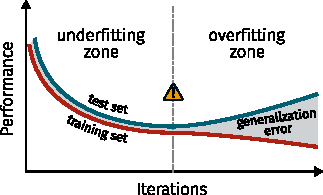
\includegraphics{graphics/overfitting-2}
    \caption[Overfitting as Function of Number of Epochs]{%
        Training a neural network model for many iterations 
        runs the risk of overfitting the model to the training data.
        Although the training error keeps decreasing, 
        it happens at the expense of increased generalization error.
    }
    \label{fig:generalization-error}
\end{marginfigure}
% }}}

\Cref{fig:generalization-error} shows a theoretical training history 
of a neural network model where the performance is calculated 
on both a training and a test set after each iteration of the training.
Here it is illustrated that 
the training loss is monotonically decreasing 
with increasing number of iterations.
The validation loss is at first also decreasing,
but if training continues for long enough,
at some point it will start to increase instead.
The divergence between training and test set performance 
indicates overfitting:
instead of learning generalizable patterns representative of the underlying 
data-generating process,
the model starts to learn or even memorise
the noise and idiosyncracies of the data that,
although characteristic in the narrow scope of the training set,
would not be representative of neither biology nor disease etiology.
~\autocite{murphyMachine2012}

Overfitting, and its counterpart, underfitting,
are key considerations in training of \ac{ML} models (\cref{fig:overfitting}).
Overfitting happens 
when a model learns the details of the training data too well, 
including the noise, 
which makes it perform poorly on unseen data.
In constrast,
underfitting occurs when the model is too simplistic 
to capture meaningful patterns in the data, 
resulting in poor performance on both the training and test sets.
Both issues highlight the need for balancing the complexity of models,
to ensure that they can effectively generalize to unobserved data.
In the section \nameref{sec:regularization},
I will outline some of the specific methods 
used to balance the complexity 
of neural network models.

% figure: overfitting {{{
\begin{figure}[htb]
    \caption[What is Overfitting?]{%
        Illustration of overfitting and underfitting 
        in a simple classification task.
        An overfitted model learns the training data too well,
        and may even remember noise and outliers,
        which makes it perform poorly on unseen data.
        Underfitted models, on the other hand,
        are to simple to capture meaningful patterns in the data.
    }
	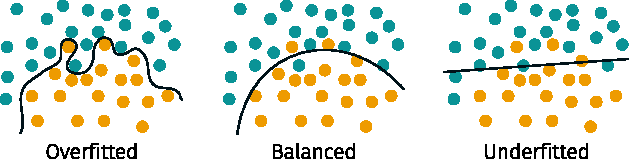
\includegraphics{graphics/overfitting}
    \label{fig:overfitting}
    \setfloatalignment{t}
    \vspace{-3em}
\end{figure}
% }}}

\section{Neural Networks}

Neural networks have been designed
using the archicteture of neurons in a human brain as inspiration.
The simplest model is that of a perceptron, 
which can be seen as a computational approximation
of a real neuron or nerve cell%
\sidenote[][-4em]{\cite{charniakIntroduction2019}}.
A typical neuron has many dendrites, a cell body, and a single axon 
(\cref{fig:neuron}).
The dendrites carries the input signal to a neuron,
and if the cumulative signal is great enough%
\sidenote[][-4em]{
    This threshold is known as 
    the \textit{threshold potential},
    and is typically between -50 and -55 mV.
}, 
then the neuron will propagate an action potential down the axon%
\sidenote[][-1em]{\cite{seifterConcepts2005}}.
In similar fashion, a perceptron receives may receive many different inputs
and produces a single output (\cref{fig:perceptron}).
In the case of a neuron, the \enquote{all-or-none} principle means
that nerve cells either signals at full strength or not all.
For a perceptron, this priniciple can be emulated
with the followingly step function:

\begin{equation}
    f_{\phi}(\bm{x})  = 
        \begin{cases}
            1 & \text{if } b + \bm{w} \cdot \bm{x} > 0\\
            0 & \text{otherwise}
        \end{cases}
\end{equation}

\begin{marginfigure}%
	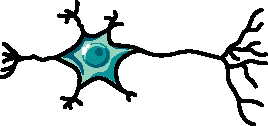
\includegraphics[width=\linewidth]{graphics/neuron}
    \caption[Schematic diagram of a neuron]{%
        Schematic diagram of a neuron.
        A typical neuron has a dendrites, a cell body, and a single axon; 
        the dendrites receive input signals from other neurons,
        and propagates output signals along the axon.
    }
    \label{fig:neuron}
\end{marginfigure}

\begin{marginfigure}%
	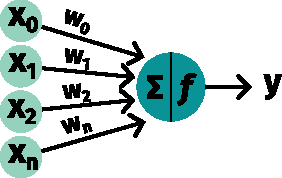
\includegraphics[width=\linewidth]{graphics/perceptron}
	\caption{Schematic diagram of a perceptron}
    \label{fig:perceptron}
\end{marginfigure}

By combing many thousands of such neurons,
in a multilayer-perceptron or artificial neural network,
we can create a model that, 
can learn even the most complex of patterns.
Deep learning is at its core a form of representation learning.
Each layer in a neural network is a different representation,
and by stacking several of such layers on top of each others,
the representation in one hidden layer
feeds into the next layer and
is thereby being transformed into an even more abstract representation%
\autocite{estevaGuide2019}.

%%%%%%%%%%%%%%%%%%%%%%%%%%%%%%%%%%%%%%%%%%%%%%%%%%%%%%%%%%%%%%%%%%%%%%%%%%%%%%%
% insert example of abstract representations in a computervis model
%%%%%%%%%%%%%%%%%%%%%%%%%%%%%%%%%%%%%%%%%%%%%%%%%%%%%%%%%%%%%%%%%%%%%%%%%%%%%%%

\section{Hyperparameter Optimization}

We can estimate the generalization error of a model
by evaluating it on a test set.
If we are only creating a single model,
then this approach suffices. 
However, we might want to compare many different models,
or slightly tweak an already existing model,
such that we can select the best performing version.
If we select the final model based on the test set alone,
we might inadvertently have biased the process,
and could, in a sense, have overfitted to the test data.
To avoid this, we need to completely hide away the test data
until we are done with training, experimenting, 
and hyperparameter optimization.
To allow this, we instead need three sets of data:

\begin{itemize}
    \item a training set to train or develop candidate models
    \item a validation set to evaluate the candidate models
        and select the best one
    \item a test set do the final unbiased evaluation of model performance
\end{itemize}

Another alternative is using the technique \textit{k}-fold cross-validation.

\section{Explaining Black Box Models}

A model is interpretable if we can inspect the model
and understand why it gave a certain output for a particular input.
An explainable model is one that can help us understand 
why a certain output was produced for a specific input.
Interpretability comes from inspecting the actual model.
Explainability can come from an external process.

Typically there is a distinction between model-based explanations
and post hoc explanations\autocite{vanderveldenExplainable2022}.
The scope of an explanation is the difference between
explanations for a complete model and
explanations for a single output.
Global explanation covers feature importance estimates 
for the entire dataset.
Local explanations, on the other hand, seeks to explain
the impact of the specific example under scrutiny.
A SHAP-waterfall plot is an example of a local explanation.
A saliency map of a chest radiograph that shows
which pixels contributed to the label \enquote{liver cancer}
is another example.

Shapley values measures the marginal contribution
of each individual feature.

One limitation of XAI models is the accuracy and relevance of explanations.
Explainability algorithms such as SHAP are only approximations
of the complete model.
In other words, the fidelity is not perfect and therefore neither
is the explanation.
However, for black-box models such as neural networks,
it is the next best thing.


\section{Regularization}
\label{sec:regularization}

One approach to avoid overfitting in neural networks
is a technique known as dropout.
At each step of model training,
a random set of nodes in the network are disabled.
In a sense, the result is a rough approximation of 
an ensemble of different networks.


Dropout introduces noise during training
and thereby forces the network to be less senstive of noise.
Hidden units trained with dropout needs to be useful 
with or without the presence of neighboring units.

%%%%%%%%%%%%%%%%%%%%%%%%%%%%%%%%%%%%%%%%%%%%%%%%%%%%%%%%%%%%%%%%%%%%%%%%%%%%%%%

\section{Miscellaneous}

In his review on artificial intelligence in medicine%
\autocite{topolHighperformance2019}, 
Eric Topol expresses his view that in the future
\blockquote{%
almost every type of clinician, ranging from specialty doctor to paramedic,
will be using AI technology, and in particular deep learning [...]
}.

The ability to predict adverse outcomes could make  
healthcare resources more efficient.

Systematic deugging and continuous monitoring and validation 
is of utmost importance if we are to release AI algorithms into the wild%
\autocite{topolHighperformance2019}.

There has been much discussion about, and there are many opinions on, 
the black-box nature of many machine learning algorithms and 
how it should or should not affect the clinical use of such 
\autocite{topolHighperformance2019, gunningXAI2019, vanderveldenExplainable2022}.

In computer vision tasks in the medical domain,
deep-learning models have achieved physician-level performance
in many different diagnostic tasks
ranging from \todo{finish sentence}.

Automated diagnosis in ophthalmology 
from optical coherence tomography scans~\autocite{defauwClinically2018}.

\section{Computational models in cardiology}

Using single-lead lectrocardiogram recordings from \num{53877} patients,
Hannun et al.\autocite{hannunCardiologistlevel2019}
constructed a deep neural network
to identify 12 difference classes of cardiac rythm.
In the validation of their algorithm on an independent test set,
the authors were able to show that the computer model
significantly outperforms the average cardiologist. 

As the amount of available diagnostic data increases,
it becomes more difficult for the treating physician
to fully utilize the complete array of phenotypic information.
Computational models can easily integrate all this data,
and through automated identification of important clinical patterns
they could serve as an important diagnostic support.

\vskip 10em

Historically, artificial neural networks (ANNs) have been predominantly
employed for classification tasks, such as those typically found 
in image recognition and natural language processing. 
However, advancements have expanded their applicability, allowing ANNs 
to be tailored for handling time-to-event data.
This extension is particularly useful in fields like healthcare and systems
biology, where survival analysis or event prediction over a time horizon is
critical. 
While the present chapter will not delve further into machine learning
applications for time-to-event data, the topic will be revisited in the
subsequent chapter.

